\chapter{Cardinality Estimation Model}
\chaptermark{Estimation Model}

\label{chap:neo4j-impl}

\begin{aboutchapter}
In this chapter, we use the query algebra defined
in Chapter \ref{chap:query-algebra} and the logical properties framework
defined in Chapter \ref{chap:log-props-framework}
to implement cardinality estimations for Neo4j.
Our estimations use a label partition and a sublabel map (cf. Section
\ref{sec:more-label-info}) as additional
information to the Neo4j statistics.
\end{aboutchapter}

\section{The Neo4j Graph Database}
\label{sec:about-neo4j}

Neo4j\footnote{\url{https://neo4j.com/}}
is a popular graph database written in Java. In Neo4j, a database consists of a
\emph{property graph}. A property graph is an extension of a labeled and typed
multigraph (cf. Definition \ref{def:database-graph}) that allows to store
properties at nodes.
Key to Neo4j's popularity is the expressive and user-friendly query language
\emph{Cypher}.

Our query algebra can be used to express an important subset of Cypher, namely
the matching of subgraphs with label, type and uniqueness constraints.

Because Neo4j is open-source software and thus easy to modify, we use
it as testbed for our cardinality estimations.

\section{Query Language Restrictions}
\label{sec:query-restrictions}

Due to three limitations, we can only provide estimations for a restricted
query space.

Firstly, the estimations developed in this thesis are tested in the JCascades
framework.
JCascades is a general Java implementation of the Cascades
framework for query optimization and is developed at the University of
Konstanz. In its current state of development it lacks support for certain
kinds of operators, including the \op{NodeJoin} operator.

Secondly, to estimate the result cardinalities of cyclic queries
(i.e., subgraph patterns containing a cycle), we
need statistics about the likeliness of cycles in the database.
Unfortunately, Neo4j currently lacks such statistics.
Implementing these statistics is not possible as part of this
work, due to limited resources and time.
Therefore we do not consider cyclic queries, i.e. queries containing
a \op{Traverse} operator.

Thirdly, in this first version of the estimations, we do not cover the
\op{DistinctSelection} operator. This is for time reasons only.

As a result, our estimations only cover the incomplete set of operators
\[
  \{ \getnodes{v}, \selection{v:l},
     \expandvar{v}{r:T}{\alpha}{w} \}
\]

The fraction of the result space covered by these operators consists of all
query results produced by non-cyclic subgraph patterns having only one
single component and no uniqueness constraints.
That is, all query results produced by \emph{tree subgraph patterns} with no
uniqueness constraints.
In Section \ref{sec:cypher-to-operators} we define the corresponding subset of
Cypher.

\section{Logical Database Properties}
\label{sec:logical-database-props}

The estimations developed in this thesis are intended to be usable in the Neo4j
graph database. Therefore, the logical database properties used in the
estimations are very similar to those available in the Neo4j statistics.

For convenience we use $*$ as a wildcard label that selects all nodes and
similarly as a wildcard relationship type that allows all relationship types.
Let $l, l_1, l_2 \in \nlabels \cup \{ * \}, t \in \rtypes \cup \{ * \}$ and
$\alpha \in \{\leftarrow, \rightarrow \}$.
The wildcard label selection is defined as $\selection{v:*}(\Omega) := \Omega$.

We require the following logical database properties $\props{G}$.
\begin{enumerate}[1.]
  \item The number of nodes in $G$ having the label $l$.
    \[
      N(l) := \card{\selection{v:l}(\getnodes{v})}
    \]
  \item The number of outgoing/incoming relationships of type $t$ in $G$
    from nodes with label $l_1$ to nodes with label $l_2$ (sometimes called
    triple statistics).
    \[
      R_\alpha(l_1, t, l_2) := \card{\selection{w:l_2}(
        \expandvar{v}{r:T}{\alpha}{w}(\selection{v:l_1}(\getnodes{v}))
        )}
    \]
    where $T := \begin{cases}
                  \rtypes \text{ if } t = *, \\
                  \{ t \}, \text{ otherwise}
                \end{cases}$.
  \item A label partition $\lpart$ as described in Section
    \ref{sub:label-partition}.
  \item A sublabel map $\submap$ as described in Section
    \ref{sub:sublabel-map}.
\end{enumerate}

Neo4j offers all of these logical database properties, but it estimates
\[
  R_\alpha(l_1, t, l_2) \approx \min \{ R_\alpha(l_1, t, *),
                                        R_\alpha(*, t, l_2) \}
\]
Our estimations require the actual values of $R_\alpha(l_1, t, l_2)$
to yield good results. Hence, we have to implement the collection of these
values. Currently this is done by executing the corresponding queries
in Neo4j and storing the result cardinalities in a CSV file.
In the future, this should be integrated into the Neo4j statistics and updated
online.

Because every relationship has exactly one type, we can obtain the number of
relationships of any type in $T \subseteq \rtypes$ and any direction $\alpha$
between nodes with label $l_1$ to nodes with label $l_2$ as
\[
  R_\alpha(l_1, T, l_2) = \sum_{t \in T} R_\alpha(l_1, t, l_2)
\]

Furthermore, we can define the average degree in $\alpha$ direction as
\[
  \avgdeg_\alpha(l_1, T, l_2) := \frac{R_\alpha(l_1, T, l_2)}{N(l_1)}
\]

\section{Logical Result Properties}
\label{sub:neo4j-log-result-props}

As described in Chapter \ref{chap:log-props-framework} the logical properties of
a query result $\Omega$ are estimated by building a chain of estimation
functions.
If the information content of the logical result properties is too small,
it can happen that the estimated properties diverge from reality for
queries incorporating many operators.

To limit this risk, we store a subgraph pattern $\rho(\Omega)$ producing the
query result in the logical properties (in Section \ref{sec:completeness} we
have shown that such a subgraph pattern exists for all query results).
From this pattern, the estimation functions know about all the previous
operators in the estimation chain.

In addition, we store for all node variables $v \in \nvars(\Omega)$ the
probability of drawing a subgraph from the query result where the node matched
by $v$ has the label $l$, $\prob{\Omega}(v{:}l)$
(cf. Equation \ref{eq:label-probability}).

We also store a Boolean flag, indicating whether the result was produced by the
\op{GetNodes} operator:
\begin{align}
  \initial(\Omega) :\Leftrightarrow \Omega = \getnodes{v}
    \text{ for some } v \in \qvars
\end{align}

Finally, the logical result properties contain the result cardinality
$\card{\Omega}$.
The memory requirements of the logical properties are shown in Table
\ref{table:neo4j-log-result-props-mem-reqs}.

\begin{table}[H]
\centering
\begin{tabular}{ll}
\toprule
Component                  & Space complexity                                                     \\ \midrule
Subgraph pattern           & $O(\binom{\card{R_\rho}}{2} + \card{V_\rho} \cdot \card{\nlabels})$
                             (cf. Table \ref{table:subgraph-pattern-mem-reqs})                    \\[3pt]
Label probabilities        & $O(\card{V_\rho} \cdot \card{\nlabels})$                             \\[3pt]
Initial flag               & $O(1)$                                                               \\[3pt]
Result cardinality         & $O(1)$                                                               \\[3pt]
\textbf{Total:}            & $O(\binom{\card{R_\rho}}{2}) + \card{V_\rho} \cdot \card{\nlabels})$ \\
\bottomrule
\end{tabular}
\caption{Space complexity of the logical result properties.}
\label{table:neo4j-log-result-props-mem-reqs}
\end{table}

\begin{remark}
From a purely logical perspective, the label probabilities, the initial flag
and the result cardinality are already determined by the subgraph pattern.

However, the logical result properties are not intended to be logically
minimal, but to allow for \emph{efficient} computations in the estimation
functions.

Deducing the exact cardinality from the subgraph pattern would often
require to execute the query, which we want to avoid.
Instead, we want a \emph{fast estimation} of the output cardinality,
which is only possible if we store logically redundant information.
\end{remark}

%TODO: rethink title
\section{Assumption About Node Degrees}
\sectionmark{Degree Assumption}

We assume node degrees are approximately uniformly distributed among
nodes with the same label, i.e. the individual node degrees are close
enough to the average degree to use it as an estimation:
For any query result $\Omega$, node variables $x, y$ and relationship
directions $\alpha \in \{ \leftarrow, \rightarrow \}$ and for any node labels
$l_1 \in \nlabels, l_2 \in \nlabels \cup \{ * \}$ we have:
\begin{align}
  \card{\selection{y:l_2}(\expandvar{x}{r:T}{\alpha}{y}(
                       \selection{x:l_1}(\Omega)
                     ))}
  \approx
    \card{\selection{x:l_1}(\Omega)} \cdot \avgdeg_\alpha(l_1, T, l_2)
  \label{ass:uniformity-1}
\end{align}

For nodes not having any label, we assume the node degree equals the overall
average node degree:
\begin{align}
  \card{\selection{y:l_2}(\expandvar{x}{r:T}{\alpha}{y}(
     \Omega \setminus \bigunion_{l_1 \in \nlabels} \selection{x:l_1}(\Omega)
  ))}
  \approx
    \card{\Omega \setminus
      \bigunion_{l_1 \in \nlabels} \selection{x:l_1}(\Omega)}
    \cdot \avgdeg_\alpha(*, T, l_2)
  \label{ass:uniformity-2}
\end{align}

\section{Estimation Functions}

An estimation function for the logical result properties of an operator $o$
takes a subgraph pattern, an initial flag, label probabilities and a cardinality
corresponding to the input and computes a new subgraph pattern, a new initial
flag, new label probabilities and a new result cardinality corresponding to the
result of $o$ (see Section \ref{sub:neo4j-log-result-props}).

We have to define such an estimation function for every operator of our
query algebra.

From the proofs that the individual operators are well-defined, we already
know how to compute the result subgraph pattern from the input subgraph
pattern for every operator (cf. Section \ref{sec:operators}).
Therefore, we only have to define functions for the initial flag, the result
cardinality and the label probabilities.

\subsection{Estimation for \op{GetNodes}}
$\getnodes{v}$ returns the set of all single node subgraphs of $G$,
matched by the variable $v$.

\paragraph{Initial flag}

The result is initial:
\begin{align}
  \initial(\getnodes{v}) \Leftrightarrow \true
\end{align}

\paragraph{Result cardinality}

The result cardinality is the number of nodes in the database:
\begin{align}
  \card{\getnodes{v}} = N(*)
\end{align}

\paragraph{Label probabilities}

The probability of drawing a node matched by $v$, having a particular label $l$
equals the fraction of nodes in the database having this label: 
\begin{align}
\begin{split}
  \prob{\getnodes{v}}(v{:}l) &= \frac{\card{\selection{v:l}(\getnodes{v})}}
                                     {\card{\getnodes{v}}} \\
                             &= \frac{N(l)}{N(*)}
\end{split}
\end{align}


\subsection{Estimation for \op{NodeLabelSelection}}

$\selection{v:l}(\Omega)$ keeps all subgraphs from $\Omega$, where the node
matched by $v$ has the label $l$.

\paragraph{Initial flag}

The result of the selection is initial, iff the input is initial and all
nodes matched by $v$ in the input have the label $l$:
\begin{align}
\begin{split}
  \initial(\selection{v:l}(\Omega))
    &\Leftrightarrow \selection{v:l}(\Omega) = \getnodes{v} \\
    &\Leftrightarrow \Omega = \getnodes{v} \land
      \frac{\card{\selection{v:l}(\getnodes{v})}}
           {\card{\getnodes{v}}} = 1 \\
    &\Leftrightarrow \initial(\Omega) \land
      \prob{\Omega}(x{:}l) = 1
\end{split}
\end{align}

\paragraph{Result cardinality}

The result cardinality of the selection is given as:
\begin{align}
\begin{split}
  \card{\selection{v:l}(\Omega)} &= \frac{\card{\selection{v:l}(\Omega)}}
                                         {\card{\Omega}}
                                    \cdot \card{\Omega} \\
                                 &= \prob{\Omega}(v{:}l) \cdot \card{\Omega}
\end{split}
\end{align}

\paragraph{Label probabilities}

We derive the new label probabilities using a case distinction.

We first look at the label probabilities at the variable $v$.
Firstly, in the result all nodes matched by $v$ have the label $l$:
\begin{align}
\begin{split}
  \prob{\selection{v:l}(\Omega)}(v{:}l)
    &= \frac{\card{\selection{v:l}(\selection{v:l}(\Omega))}}
            {\card{\selection{v:l}(\Omega)}} \\
    &= \frac{\card{\selection{v:l}(\Omega)}}
            {\card{\selection{v:l}(\Omega)}} \\
    &= 1
\end{split}
\end{align}
The same holds for all nodes matched by $v$ having a superlabel of $l$, i.e.,
$\prob{\selection{v:l}(\Omega)}(v{:}l') = 1$ if $l \in \submap(l')$.

Now take a label $l' \in \nlabels, l' \not = l$. If
$\lpart(l') \not = \lpart(l)$, then we assume the labels are disjoint and we
have
\begin{align}
\begin{split}
  \prob{\selection{v:l}(\Omega)}(v{:}l')
    &= \frac{\card{\selection{v:l'}(\selection{v:l}(\Omega))}}{\card{\selection{v:l}(\Omega)}} \\
    &= \frac{\prob{\Omega}(v{:}l' \isect v{:}l)}{\prob{\Omega}(v{:}l)} \\
    &\approx 0
\end{split}
\end{align}

Else, if $l' \in s(l)$, then we assume that $l'$ is a sublabel of $l$:
\begin{align}
\begin{split}
  \prob{\selection{v:l}(\Omega)}(v{:}l')
    &= \frac{\prob{\Omega}(v{:}l' \isect v{:}l)}{\prob{\Omega}(v{:}l)} \\
    &\approx \frac{\prob{\Omega}(v{:}l')}{\prob{\Omega}(v{:}l)}
\end{split}
\end{align}

Else, we assume that $l$ and $l'$ are independent in $\Omega$:
\begin{align}
\begin{split}
  \prob{\selection{v:l}(\Omega)}(v{:}l')
    &= \frac{\prob{\Omega}(v{:}l' \isect v{:}l)}{\prob{\Omega}(v{:}l)} \\
    &\approx \frac{\prob{\Omega}(v{:}l') \cdot \prob{\Omega}(v{:}l)}{\prob{\Omega}(v{:}l)} \\
    &= \prob{\Omega}(v{:}l')
\end{split}
\end{align}

Now take a node variable $v'$ with $v' \not = v$.
The problem is to compute the expression
\begin{align}
\begin{split}
  \prob{\selection{v:l}(\Omega)}(v'{:}l')
    &= \frac{\prob{\Omega}(v'{:}l' \isect v{:}l)}{\prob{\Omega}(v{:}l)} \\
\end{split}
\end{align}
This is impossible without exploiting information about how $v$ and
$v'$ are connected in the subgraph pattern $\rho$.
Although we have this information available from $\rho$ in theory, using it
would require potentially costly traversals of the pattern and significantly
increase the amount of time required to compute the new label probabilities.

Instead, we assume that the events $v'{:}l'$ and $v{:}l$ are independent in
$\Omega$, i.e., that selecting a label on one node variable of a pattern does
not affect the distribution of labels at other node variables of this pattern:
\begin{align}
\begin{split}
  \prob{\selection{v:l}(\Omega)}(v'{:}l') \approx \prob{\Omega}(v'{:}l')
\end{split}
\end{align}

\begin{remark}
This assumption somehow contradicts the motivation of the thesis, because it
neglects the possibility of strong correlations between the existence of
relationships between nodes and the labels of these nodes.

In future revisions of this work another solution might be proposed.
However, the current assumption allows for very local updates to the
label probabilities (only the probabilities at the variable $v$ must be
updated) and can therefore be computed very fast.

Also note that, correlations between relationship types and labels are
considered in the estimation functions of the \op{Expand} operator.
\end{remark}

\subsection{Estimation for \op{Expand}}

$\expandvar{x}{r:T}{\alpha}{y}(\Omega)$ expands the subgraphs in $\Omega$
by matching relationships $r$ of types $T$ starting at nodes matched by $x$
and going to nodes matched by $y$ in direction $\alpha$.

\paragraph{Initial flag}

The result of an expand is never initial:
\begin{align*}
  \initial(\expandvar{x}{r:T}{\alpha}{y}(\Omega))
    &\Leftrightarrow \expandvar{x}{r:T}{\alpha}{y}(\Omega) = \getnodes{x} \\
    &\Rightarrow \rvars(\expandvar{x}{r:T}{\alpha}{y}(\Omega))
                 = \rvars(\getnodes{x}) \\
    &\Rightarrow \{ r \} \subseteq \emptyset \\
    &\Leftrightarrow \false
\end{align*}

\paragraph{Result cardinality}

If the input $\Omega$ is initial, i.e. it is the result of a \op{GetNodes}
operator, we know the exact result cardinality from the database properties:
\begin{align}
  \card{\expandvar{x}{r:T}{\alpha}{y}(\getnodes{x})} = R_\alpha(*, T, *)
\end{align}

Let us now focus on the case where $\Omega$ is not initial.
The idea of the estimation function for the result cardinality is to
describe the nodes matched by the variable $v$ in $\Omega$
in terms of their node labels.

Because there is only a finite number of labels in the database, we can
enumerate them according to the partition of overlapping labels:
Let $\lpart_i$ be the $i$-th member set of $\lpart$ and
$l_{i,j}$ the $j$-th label in $\lpart_i$.

For each node, \emph{one} node label $l$ is chosen that is considered to be
most representative for this node.
The degree of the node is then estimated as the average degree
$\avgdeg_\alpha(l, T, *)$ of all nodes having this representative label.
The assignment of nodes to representative labels happens using the information
stored in the input label probabilities, the label partition $\lpart$ and the
sublabel map $\submap$.

\vspace{1em}
In the first step, we divide the set of input subgraphs into two subsets.
In the first subset, we put those subgraphs where the nodes matched by $x$
have any label. In the second subset, we put the subgraphs where the nodes
matched by $x$ have no label:
\begin{align}
\begin{split}
  \card{\expandvar{x}{r:T}{\alpha}{y}(\Omega)}
               = &\card{\expandvar{x}{r:T}{\alpha}{y}(
                    \bigunion_{l \in \nlabels} \selection{x:l}(\Omega))}
                      ~~\text{(1)} \\
                   &+ \\
                   &\card{\expandvar{x}{r:T}{\alpha}{y}(
                     \Omega \setminus
                       \bigunion_{l \in \nlabels} \selection{x:l}(\Omega))}
                         ~~\text{(2)}
\end{split}
\end{align}

We now rewrite the first term as a sum over the member sets of the node label
partition $\lpart$. After that, we add an inner sum over the
respective node labels of each member set.
For each node label $l_{i,j} \in \lpart_i$, we count the
number of subgraphs produced by the expand applied on the nodes in $\Omega$
which have the label $l_{i,j}$, but do not have any of the labels
$l_{i,1}, \ldots, l_{i, j-1}$.
These nodes are then considered to be best represented by the label $l_{i,j}$.
Therefore, their degree is estimated as $\avgdeg_\alpha(l_{i,j}, T, *)$, using
the degree uniformity assumption. This gives us the following result:
\begin{align}
\begin{split}
  \text{(1)} &= \card{\expandvar{x}{r:T}{\alpha}{y}(\bigunion_{l \in \nlabels} \selection{x:l}(\Omega))} \\
             &\approx \sum_{i=1}^\card{\lpart}
                  \card{\expandvar{x}{r:T}{\alpha}{y}(\bigunion_{j=1}^\card{\lpart_i}
                  \selection{x:l_{i,j}}(\Omega))} \\
             &= \sum_{i=1}^\card{\lpart}
                \sum_{j=1}^\card{\lpart_i}
                  \card{\expandvar{x}{r:T}{\alpha}{y}(\selection{x:l_{i,j}}(
                  \Omega \setminus \bigunion_{k=1}^{j-1} \selection{x:l_{i,k}}(\Omega)
                  ))} \\
            \text{\tiny Equation \ref{ass:uniformity-1}} &\omit\dotfill \\
             &\approx \sum_{i=1}^\card{\lpart}
                      \sum_{j=1}^\card{\lpart_i}
                        \card{\selection{x:l_{i,j}}(
                        \Omega \setminus \bigunion_{k=1}^{j-1} \selection{x:l_{i,k}}(\Omega)
                        )}
                        \cdot \avgdeg_\alpha(l_{i,j}, T, *) \\
             &= \sum_{i=1}^\card{\lpart}
                \sum_{j=1}^\card{\lpart_i}
                  \card{\Omega}
                  \cdot \prob{\Omega}(x{:}l_{i,j} \isect \overline{\bigunion_{k=1}^{j-1} x{:}l_{i,k}})
                  \cdot \avgdeg_\alpha(l_{i,j}, T, *) \\
             &= \card{\Omega}
                \cdot
                \sum_{i=1}^\card{\lpart}
                \sum_{j=1}^\card{\lpart_i}
                  \prob{\Omega}(x{:}l_{i,j} \isect \bigisect_{k=1}^{j-1} \overline{x{:}l_{i,k}})
                  \cdot \avgdeg_\alpha(l_{i,j}, T, *)
\end{split}
\end{align}

At this point, we want to highlight a strength of our approach:
By taking into account the label probabilities of the input, the estimations
are precise even if there are strong dependencies between labels and the
presence of relationships.
If e.g., the input consists only of nodes having exactly one particular label,
then only the average degree of nodes of this label is used to estimate the
result cardinality.
Neo4j does not track label probabilities and is therefore unable to deal with
such dependencies.

The remaining problem is to sensibly estimate
$\prob{\Omega}(x{:}l_{i,j} \isect
               \bigisect_{k=1}^{j-1} \overline{x{:}l_{i,k}})$, which is the
fraction of subgraphs in $\Omega$ where the nodes matched by $x$ have the label
$l_{i,j}$ but none of the labels $l_{i,1}, \ldots, l_{i,j-1}$.

We observe that, if a node has several labels, the representative label is the
one that comes first in the ordering in the member set of the label partition.
Consequently, this ordering plays an essential role in the quality of the
estimation function.

A simple approach is to sort the labels $l$ descendingly by the product
$\sprob(l) \cdot \frac{1}{N(l)}$. This puts the labels in front that cover
most of the nodes matched by $x$ in $\Omega$ and whose number
of nodes in the database is closest to $\Omega$. If this value is similar for
two different labels, the label $l$ with higher $\sprob(l)$ comes first in the
ordering.
We will use this ordering for the estimation function.

\begin{remark}
This simple approach does not take into account that nodes can be
matched several times by the same variable $x$ in different subgraphs of
$\selection{x:l}(\Omega)$.
It can happen that $x$ matches only one single node in the database in all
subgraphs of $\Omega$ while $\sprob(l) = 1$ and $N(l) = \card{\Omega}$.
In this case, the risk of an estimation error is very high, because it is
probable that this single node having label $l$ behaves differently than
a larger sample of nodes having $l$.

This problem could be addressed by sorting the labels according to a similarity
measure that describes the cardinality of the intersection of the nodes
matched by $x$ in $\selection{x:l}(\Omega)$ and in
$\selection{x:l}(\getnodes{x})$.
However, such a similarity measure would require storing and updating
information about the uniqueness of nodes matched by a particular node variable
and having a particular label.
\end{remark}

Now that we have discussed the ordering, we will present a solution for
computing
$\prob{\Omega}(x{:}l_{i,j}
       \isect \bigisect_{k=1}^{j-1} \overline{x{:}l_{i,k}})$.

To make the equations more readable, we write $\sprob$ for $\prob{\Omega}$.

Take a partition member set $\lpart_i \in \lpart$ and a subset of labels
$L \subset \lpart_i$. Take one label $l \in \lpart_i \setminus L$.

It holds that
\begin{align}
\begin{split}
  \sprob(l \isect \bigisect_{l' \in L} \overline{l'})
    &= \sprob(l \mid \bigisect_{l' \in L} \overline{l'})
       \cdot \sprob(\bigisect_{l' \in L} \overline{l'}) \\
    &= (1 - \sprob(\overline{l} \mid \bigisect_{l' \in L} \overline{l'}))
       \cdot \sprob(\bigisect_{l' \in L} \overline{l'}) \\
    &= (1 - \frac{\sprob(\bigisect_{l' \in L \union \{l\}} \overline{l'})}
                 {\sprob(\bigisect_{l' \in L} \overline{l'})})
       \cdot \sprob(\bigisect_{l' \in L} \overline{l'}) \\
    &= \sprob(\bigisect_{l' \in L} \overline{l'})
       - \sprob(\bigisect_{l' \in L \union \{l\}} \overline{l'})
    \label{eq:label-prob-1}
\end{split}
\end{align}

Take again a subset of labels $L \subset \lpart_i$ and a label
$l \in \lpart_i \setminus L$. For all $l' \in L$ that are sublabels
of $l$, the probability of drawing a node that does neither have the label
$l$ nor the label $l'$ equals the probability of drawing a node that does
not have the label $l$:
\begin{align*}
  \sprob(\overline{l} \isect \overline{l'}) \approx \sprob(\overline{l})
\end{align*}

Consequently, let $S := (L \setminus \submap(l)) \union \{l\}$. We have
\begin{align}
\begin{split}
  \sprob(\bigisect_{l' \in L \union \{l\}} \overline{l'})
    &\approx \sprob(\bigisect_{l' \in S \union \{l\}} \overline{l'})
    \label{eq:label-prob-2}
\end{split}
\end{align}

Iterative application of Equation \ref{eq:label-prob-2} gives us a minimal
set of superlabels $S^*$. For all $l \in S^*$, no sublabel of $l$ is contained
in $S^*$, i.e., $S^* \isect \submap(l) = \emptyset$.
For this set of superlabels we assume independence and obtain
\begin{align}
  \sprob(\bigisect_{l' \in S^*} \overline{l'})
    \approx \prod_{l' \in S^*} 1 - \sprob(l')
  \label{eq:label-prob-3}
\end{align}

Together, the Equations \ref{eq:label-prob-1} and \ref{eq:label-prob-3}
provide an easily computable, recursive estimation of
$\prob{\Omega}(x{:}l \isect \bigisect_{l' \in L} \overline{x{:}l'})$.


For the second term we apply the same technique:
\begin{align}
\begin{split}
  \text{(2)} &= \card{\expandvar{x}{r:T}{\alpha}{y}(
                      \Omega \setminus
                        \bigunion_{l \in \nlabels} \selection{x:l}(\Omega))} \\
            \text{\tiny Equation \ref{ass:uniformity-2}} &\omit\dotfill \\
             &\approx
                \card{\Omega \setminus
                        \bigunion_{l \in \nlabels} \selection{x:l}(\Omega)}
                \cdot \avgdeg_\alpha(*,T,*) \\
             &= \card{\Omega}
                \cdot \prob{\Omega}(\overline{\bigunion_{l \in \nlabels} x{:}l})
                \cdot \avgdeg_\alpha(*,T,*) \\
             &= \card{\Omega}
                \cdot (1 - \prob{\Omega}(\bigisect_{l \in \nlabels} x{:}l))
                \cdot \avgdeg_\alpha(*,T,*)
\end{split}
\end{align}

From Equation \ref{eq:label-prob-3} we know how to recursively compute the probability
expression in this formula.

\begingroup
\newcommand{\estDeg}{\textit{estDeg}}
\newcommand{\remaining}{\textit{remaining}}
\newcommand{\oldRemaining}{\textit{oldRemaining}}
\newcommand{\newRemaining}{\textit{newRemaining}}
\newcommand{\superLabels}{\textit{superLabels}}
\newcommand{\coveredLabels}{\textit{coveredLabels}}
\newcommand{\notCoveredBySuperLabels}{\textit{notCoveredBySuperLabels}}
\newcommand{\changed}{\textit{changed}}

To demonstrate the computability of the expand estimations,
we use Algorithm \ref{algo:expand-cardinality} that computes both terms (1)
and (2) in a single loop over the set of node labels.

The most interesting variables are the following:
\begin{itemize}
  \item $\estDeg$ stores the amount contributed to the total estimated degree
    by the nodes having one of the already covered labels ($\coveredLabels$).

  \item $\remaining$ stores the fraction of nodes matched by $v$ whose degree
    has not yet been estimated. After the loop has finished, this variable
    stores the fraction of nodes matched by $v$ not having any label, which
    allows to compute (2).

  \item $\superLabels$ stores the current minimal set of superlabels, as
    defined above. It is updated once in each iteration.

  \item $\notCoveredBySuperLabels$ stores the fraction of nodes matched by $v$
    that does not have any of these superlabels. If the minimal set of
    superlabels changes because of the current label, this variable has to be
    recomputed as a product over all superlabels.
    Otherwise, the cached value of the last iteration can be used and only a
    single multiplication is needed.
\end{itemize}

\begin{algorithm}
  \caption{{\sc computeExpandCardinality}}
  \label{algo:expand-cardinality}
  \DontPrintSemicolon
  \KwIn{$\estprops{\Omega}$ (estimation of the logical result properties of
        $\Omega$), $\props{G}$ (logical database properties)}
  \KwOut{estimation of $\card{\expandvar{x}{r:T}{\alpha}{y}(\Omega)}$}
  
  \eIf{$\initial(\Omega)$}{
      \tcp*[l]{We know the exact cardinality from the database properties.}
      \Return $R_\alpha(*, T, *)$\;
  }{
    \tcp*[l]{We estimate the cardinality by combining the node degrees for
             the different labels.}
    $\estDeg \gets 0$\;
    $\remaining \gets 1$\;
    
    \BlankLine
    \tcp*[l]{(1) Estimate the node degree for nodes having a label.}
    
    $i \gets 1$\;
    \While{$i < \card{\lpart} \land \remaining > 0$}{
      \tcp*[l]{Outer sum over the partition member sets.}
      
      $\oldRemaining \gets \remaining$\;
      $\superLabels \gets \emptyset$\;
      $\notCoveredBySuperLabels \gets 1$\;
      $\coveredLabels \gets \emptyset$\;
      
      $j \gets 1$\;
      \While{$j < \card{\lpart_i} \land \remaining > 0$}{
        \tcp*[l]{Inner sum over the labels in a partition member set.}
        
        \If{$l_{i,j} \not \in \coveredLabels$}{
          $\superLabels \gets (\superLabels \setminus \submap(l_{i,j}))$\;
          $\changed \gets \text{ whether } \superLabels \text{ has changed}$\;
          $\superLabels \gets \superLabels \union \{l_{i,j}\}$\;
          
          \eIf{$\changed$}{
            $\notCoveredBySuperLabels
              \gets \prod_{l \in \superLabels} 1 - \prob{\Omega}(x{:}l)$\;
          }{
            $\notCoveredBySuperLabels
              \gets \notCoveredBySuperLabels
                \cdot (1 - \prob{\Omega}(x{:}l_{i,j}))$\;
          }
        
          $\newRemaining \gets
            \notCoveredBySuperLabels - (1 - \oldRemaining)$\;
          
          $\estDeg \gets \estDeg + \avgdeg_\alpha(l_{i,j}, T, *)
            \cdot (\remaining - \newRemaining)$\;
          
          $\remaining \gets \newRemaining$\;
        }
        $\coveredLabels \gets \coveredLabels \union \submap(l_{i,j})$\;
        
        $j \gets j + 1$\;
      }
      $i \gets i + 1$\;
    }
    
    \BlankLine
    \tcp*[l]{(2) Estimate the node degree for nodes having no label.}
    
    $\estDeg \gets \estDeg + \avgdeg_\alpha(*, T, *) \cdot \remaining$\;
    
    \BlankLine
    \tcp*[l]{Compute the result cardinality.}
    
    \Return $\card{\Omega} \cdot \estDeg$\;
  }
\end{algorithm}

To better understand this algorithm, recall the example database about movies
and its distribution of node labels shown in Figure
\ref{fig:label-dist-example}.

In Figure \ref{fig:label-dist-example-with-result} we add to this diagram the
set of nodes matched by the variable $v$ of some query result $\Omega$.
Note that the size of the area does not necessarily
correspond to the cardinality of $\Omega$, as nodes can be matched several
times by the same variable in different subgraphs.

\begin{figure}
  \centering
  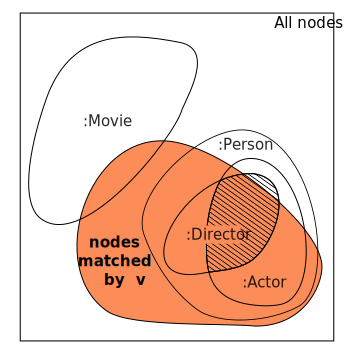
\includegraphics[width=0.4\textwidth]{figures/nodes-venn-diagram-with-query-result.pdf}
  \caption{Distribution of node labels and a query result in a example
           database.}
  \label{fig:label-dist-example-with-result}
\end{figure}

The outer loop of the algorithm iterates over the member sets of the label
partition. The inner loop iterates over the labels of one member set.
The order is given by the indices of the label variable $l_{i,j}$.
Suppose the algorithm iterates over the label partition in the following
order:
\begin{align*}
  l_{1,1} = \text{Movie} \\
  l_{2,1} = \text{Actor} \\
  l_{2,2} = \text{Director} \\
  l_{2,3} = \text{Person}
\end{align*}

We write again $\sprob(l)$ instead of $\prob{\Omega}(v{:}l)$ for better
readability.
The trace of the algorithm execution of the example is given by Table
\ref{table:expand-cardinality-trace-1} and Table
\ref{table:expand-cardinality-trace-2}.
Reading the tables from top to bottom we can see all variable assignments
performed by the algorithm in chronological order.
The column $l_{i,j}$ shows, which label is currently used to estimate the
degree of a fraction of the matched nodes.

Figure \ref{fig:expand-cardinality-steps} shows the usage of representative
labels for the nodes matched by $v$ as a sequence of Venn diagrams.
In each diagram, the orange area represents the fraction of nodes whose degree
is estimated in the current iteration of the algorithm.
The result of this estimation is written below the diagram (cf. the trace
of the algorithm in Table \ref{table:expand-cardinality-trace-1} and
Table \ref{table:expand-cardinality-trace-2}).
The total estimated degree of the nodes matched by $v$ is the sum of all the
partial degrees shown in the individual diagrams.

\begin{figure}
  \centering
  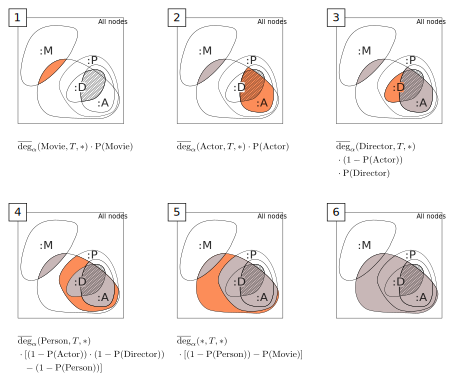
\includegraphics[width=\textwidth]{figures/labels-for-estimation-step-by-step-complete-formulas.pdf}
  \caption{Step-by-step visualization of the expand cardinality estimation.
           \textit{Orange:} The fraction of nodes whose degree is currently estimated.
           \textit{Grey:} Already covered fraction of nodes.
           \textit{Below each diagram:} The estimated degree corresponding to the orange fraction.}
  \label{fig:expand-cardinality-steps}
\end{figure}

\begin{landscape}
  \begin{table}[]
\vspace{-\marginparsep}
\vspace{-\marginparwidth}

\centering
\caption{Trace of the \textsc{ComputeExpandCardinality} algorithm (1).}
\label{table:expand-cardinality-trace-1}

\resizebox{\columnwidth}{!}{%
\begin{tabular}{lllllllllll}
$i$                       & $j$                       & $l_{i,j}$         & \estDeg                                                                  & \remaining                                                             & \oldRemaining             & \superLabels                                                & \coveredLabels                                                             & \notCoveredBySuperLabels                                                  & \changed                        & \newRemaining                                                          \\
                          &                           &                   & \cellcolor[HTML]{FC8D59}$0$                                              &                                                                        &                           &                                                             &                                                                            &                                                                           &                                 &                                                                        \\
                          &                           &                   &                                                                          & \cellcolor[HTML]{FC8D59}$1$                                            &                           &                                                             &                                                                            &                                                                           &                                 &                                                                        \\
\cellcolor[HTML]{FC8D59}1 &                           &                   &                                                                          &                                                                        &                           &                                                             &                                                                            &                                                                           &                                 &                                                                        \\
                          &                           &                   &                                                                          &                                                                        & \cellcolor[HTML]{FC8D59}1 &                                                             &                                                                            &                                                                           &                                 &                                                                        \\
                          &                           &                   &                                                                          &                                                                        &                           & \cellcolor[HTML]{FC8D59}$\emptyset$                         &                                                                            &                                                                           &                                 &                                                                        \\
                          &                           &                   &                                                                          &                                                                        &                           &                                                             &                                                                            & \cellcolor[HTML]{FC8D59}$1$                                               &                                 &                                                                        \\
                          &                           &                   &                                                                          &                                                                        &                           &                                                             & \cellcolor[HTML]{FC8D59}$\emptyset$                                        &                                                                           &                                 &                                                                        \\
                          & \cellcolor[HTML]{FC8D59}1 & \textbf{Movie}    &                                                                          &                                                                        &                           &                                                             &                                                                            &                                                                           &                                 &                                                                        \\
                          &                           &                   &                                                                          &                                                                        &                           & \cellcolor[HTML]{FC8D59}$\emptyset$                         &                                                                            &                                                                           &                                 &                                                                        \\
                          &                           &                   &                                                                          &                                                                        &                           &                                                             &                                                                            &                                                                           & \cellcolor[HTML]{FC8D59}$false$ &                                                                        \\
                          &                           &                   &                                                                          &                                                                        &                           & \cellcolor[HTML]{FC8D59}$\{\text{Movie}\}$                  &                                                                            &                                                                           &                                 &                                                                        \\
                          &                           &                   &                                                                          &                                                                        &                           &                                                             &                                                                            & \cellcolor[HTML]{FC8D59}$1 - \sprob(\text{Movie})$
  &                                 &                                                                        \\
                          &                           &                   &                                                                          &                                                                        &                           &                                                             &                                                                            &                                                                           &                                 & \cellcolor[HTML]{FC8D59}\input{tables/expand-trace/remaining_m.tex}    \\
                          &                           &                   & \cellcolor[HTML]{FC8D59}$\avgdeg_\alpha(\text{Movie}, T, *) \cdot \sprob(\text{Movie})$
    &                                                                        &                           &                                                             &                                                                            &                                                                           &                                 &                                                                        \\
                          &                           &                   &                                                                          & \cellcolor[HTML]{FC8D59}\input{tables/expand-trace/remaining_m.tex}    &                           &                                                             &                                                                            &                                                                           &                                 &                                                                        \\
                          &                           &                   &                                                                          &                                                                        &                           &                                                             & \cellcolor[HTML]{FC8D59}$\{\text{Movie}\}$                                 &                                                                           &                                 &                                                                        \\
                          & \cellcolor[HTML]{FC8D59}2 &                   &                                                                          &                                                                        &                           &                                                             &                                                                            &                                                                           &                                 &                                                                        \\
\cellcolor[HTML]{FC8D59}2 &                           &                   &                                                                          &                                                                        &                           &                                                             &                                                                            &                                                                           &                                 &                                                                        \\
                          &                           &                   &                                                                          &                                                                        &                           &                                                             &                                                                            &                                                                           &                                 &                                                                        \\
                          &                           &                   &                                                                          &                                                                        &                           & \cellcolor[HTML]{FC8D59}$\emptyset$                         &                                                                            &                                                                           &                                 &                                                                        \\
                          &                           &                   &                                                                          &                                                                        &                           &                                                             &                                                                            & \cellcolor[HTML]{FC8D59}$1$                                               &                                 &                                                                        \\
                          &                           &                   &                                                                          &                                                                        &                           &                                                             & \cellcolor[HTML]{FC8D59}$\emptyset$                                        &                                                                           &                                 &                                                                        \\
                          & \cellcolor[HTML]{FC8D59}1 & \textbf{Actor}    &                                                                          &                                                                        &                           &                                                             &                                                                            &                                                                           &                                 &                                                                        \\
                          &                           &                   &                                                                          &                                                                        &                           &                                                             &                                                                            & \cellcolor[HTML]{FC8D59}$1$                                               &                                 &                                                                        \\
                          &                           &                   &                                                                          &                                                                        &                           & \cellcolor[HTML]{FC8D59}$\emptyset$                         &                                                                            &                                                                           &                                 &                                                                        \\
                          &                           &                   &                                                                          &                                                                        &                           &                                                             &                                                                            &                                                                           & \cellcolor[HTML]{FC8D59}$false$ &                                                                        \\
                          &                           &                   &                                                                          &                                                                        &                           & \cellcolor[HTML]{FC8D59}$\{\text{Actor}\}$                  &                                                                            &                                                                           &                                 &                                                                        \\
                          &                           &                   &                                                                          &                                                                        &                           &                                                             &                                                                            & \cellcolor[HTML]{FC8D59}$1 - \sprob(\text{Actor})$
  &                                 &                                                                        \\
                          &                           &                   &                                                                          &                                                                        &                           &                                                             &                                                                            &                                                                           &                                 & \cellcolor[HTML]{FC8D59}$\!\begin{aligned}
  &(1 - \sprob(\text{Actor})) \\
  &- \sprob(\text{Movie})
\end{aligned}$
   \\
                          &                           &                   & \cellcolor[HTML]{FC8D59}$\!\begin{aligned}
  &\avgdeg_\alpha(\text{Movie}, T, *) \cdot \sprob(\text{Movie}) \\
  &+ \avgdeg_\alpha(\text{Actor}, T, *) \cdot \sprob(\text{Actor})
\end{aligned}$
    &                                                                        &                           &                                                             &                                                                            &                                                                           &                                 &                                                                        \\
                          &                           &                   &                                                                          & \cellcolor[HTML]{FC8D59}$\!\begin{aligned}
  &(1 - \sprob(\text{Actor})) \\
  &- \sprob(\text{Movie})
\end{aligned}$
   &                           &                                                             &                                                                            &                                                                           &                                 &                                                                        \\
                          &                           &                   &                                                                          &                                                                        &                           &                                                             & \cellcolor[HTML]{FC8D59}$\{\text{Actor}\}$                                 &                                                                           &                                 &                                                                        \\
\end{tabular}%
}
\end{table}

  \begin{table}[]
\vspace{-\marginparsep}
\vspace{-\marginparwidth}

\centering
\caption{Trace of the \textsc{ComputeExpandCardinality} algorithm (2).}
\label{table:expand-cardinality-trace-2}

\resizebox{\columnwidth}{!}{%
\begin{tabular}{lllllllllll}
$i$                       & $j$                       & $l_{i,j}$         & \estDeg                                                                  & \remaining                                                             & \oldRemaining             & \superLabels                                                & \coveredLabels                                                             & \notCoveredBySuperLabels                                                  & \changed                        & \newRemaining                                                          \\
                          & \cellcolor[HTML]{FC8D59}2 & \textbf{Director} &                                                                          &                                                                        &                           &                                                             &                                                                            &                                                                           &                                 &                                                                        \\
                          &                           &                   &                                                                          &                                                                        &                           & \cellcolor[HTML]{FC8D59}$\{\text{Actor}\}$                  &                                                                            &                                                                           &                                 &                                                                        \\
                          &                           &                   &                                                                          &                                                                        &                           &                                                             &                                                                            &                                                                           & \cellcolor[HTML]{FC8D59}$false$ &                                                                        \\
                          &                           &                   &                                                                          &                                                                        &                           & \cellcolor[HTML]{FC8D59}$\{\text{Actor}, \text{Director}\}$ &                                                                            &                                                                           &                                 &                                                                        \\
                          &                           &                   &                                                                          &                                                                        &                           &                                                             &                                                                            & \cellcolor[HTML]{FC8D59}$\!\begin{aligned}
  &(1 - \sprob(\text{Actor})) \\
  &\cdot (1 - \sprob(\text(Director)))
\end{aligned}$
 &                                 &                                                                        \\
                          &                           &                   &                                                                          &                                                                        &                           &                                                             &                                                                            &                                                                           &                                 & \cellcolor[HTML]{FC8D59}$\!\begin{aligned}
  &(1 - \sprob(\text{Actor})) \\
  &~~\cdot (1 - \sprob(\text{Director})) \\
  &- \sprob(\text{Movie})
\end{aligned}$
  \\
                          &                           &                   & \cellcolor[HTML]{FC8D59}$\!\begin{aligned}
  &\avgdeg_\alpha(\text{Movie}, T, *) \cdot \sprob(\text{Movie}) \\
  &+ \avgdeg_\alpha(\text{Actor}, T, *) \cdot \sprob(\text{Actor}) \\
  &+ \avgdeg_\alpha(\text{Director}, T, *) \\
  &~~\cdot (1 - \sprob(\text{Actor})) \cdot \sprob(\text{Director})
\end{aligned}$
 &                                                                        &                           &                                                             &                                                                            &                                                                           &                                 &                                                                        \\
                          &                           &                   &                                                                          & \cellcolor[HTML]{FC8D59}$\!\begin{aligned}
  &(1 - \sprob(\text{Actor})) \\
  &~~\cdot (1 - \sprob(\text{Director})) \\
  &- \sprob(\text{Movie})
\end{aligned}$
  &                           &                                                             &                                                                            &                                                                           &                                 &                                                                        \\
                          &                           &                   &                                                                          &                                                                        &                           &                                                             & \cellcolor[HTML]{FC8D59}$\{\text{Actor}, \text{Director}\}$                &                                                                           &                                 &                                                                        \\
                          & \cellcolor[HTML]{FC8D59}3 & \textbf{Person}   &                                                                          &                                                                        &                           &                                                             &                                                                            &                                                                           &                                 &                                                                        \\
                          &                           &                   &                                                                          &                                                                        &                           & \cellcolor[HTML]{FC8D59}$\emptyset$                         &                                                                            &                                                                           &                                 &                                                                        \\
                          &                           &                   &                                                                          &                                                                        &                           &                                                             &                                                                            &                                                                           & \cellcolor[HTML]{FC8D59}$true$  &                                                                        \\
                          &                           &                   &                                                                          &                                                                        &                           & \cellcolor[HTML]{FC8D59}$\{\text{Person}\}$                 &                                                                            &                                                                           &                                 &                                                                        \\
                          &                           &                   &                                                                          &                                                                        &                           &                                                             &                                                                            & \cellcolor[HTML]{FC8D59}$1 - \sprob(\text{Person})$
  &                                 &                                                                        \\
                          &                           &                   &                                                                          &                                                                        &                           &                                                             &                                                                            &                                                                           &                                 & \cellcolor[HTML]{FC8D59}$\!\begin{aligned}
  &(1 - \sprob(\text{Person})) \\
  &- \sprob(\text{Movie})
\end{aligned}$
 \\
                          &                           &                   & \cellcolor[HTML]{FC8D59}\input{tables/expand-trace/persons_degree.tex}   &                                                                        &                           &                                                             &                                                                            &                                                                           &                                 &                                                                        \\
                          &                           &                   &                                                                          & \cellcolor[HTML]{FC8D59}$\!\begin{aligned}
  &(1 - \sprob(\text{Person})) \\
  &- \sprob(\text{Movie})
\end{aligned}$
 &                           &                                                             &                                                                            &                                                                           &                                 &                                                                        \\
                          &                           &                   &                                                                          &                                                                        &                           &                                                             & \cellcolor[HTML]{FC8D59}$\{\text{Actor}, \text{Director}, \text{Person}\}$ &                                                                           &                                 &                                                                        \\
                          & \cellcolor[HTML]{FC8D59}4 &                   &                                                                          &                                                                        &                           &                                                             &                                                                            &                                                                           &                                 &                                                                        \\
\cellcolor[HTML]{FC8D59}3 &                           &                   &                                                                          &                                                                        &                           &                                                             &                                                                            &                                                                           &                                 &                                                                        \\
                          &                           &                   & \cellcolor[HTML]{FC8D59}$\!\begin{aligned}
  &\avgdeg_\alpha(\text{Movie}, T, *) \cdot \sprob(\text{Movie}) \\
  &+ \avgdeg_\alpha(\text{Actor}, T, *) \cdot \sprob(\text{Actor}) \\
  &+ \avgdeg_\alpha(\text{Director}, T, *) \\
  &~~\cdot (1 - \sprob(\text{Actor})) \cdot \sprob(\text{Director}) \\
  &+ \avgdeg_\alpha(\text{Person}, T, *) \\
  &~~\cdot [(1 - \sprob(\text{Actor})) \\
  &~~~~\cdot (1 - \sprob(\text{Director})) - (1 - \sprob(\text{Person}))] \\
  &+ \avgdeg_\alpha(*, T, *) \\
  &~~\cdot [(1 - \sprob(\text{Person})) - \sprob(\text{Movie})]
\end{aligned}$
    &                                                                        &                           &                                                             &                                                                            &                                                                           &                                 &                                                                       
\end{tabular}%
}
\end{table}

\end{landscape}

In the beginning, the counter of the outer loop of the algorithm points to
the first partition member set of the label partition.
The counter of the inner loop points to the first label in this member set,
which is $l_{1,1} = \text{Movie}$.
The algorithm now estimates the amount contributed to the total degree
by nodes having the "Movie" label.
In Diagram 1 in Figure \ref{fig:expand-cardinality-steps} the area
corresponding to these movie nodes is highlighted in orange.
The algorithm correctly estimates the fraction of these nodes as
$\sprob(\text{Movie})$.
For any movie node, the algorithm assumes a degree of
$\avgdeg_\alpha(l_{1,1}, T, *) = \avgdeg_\alpha(\text{Movie}, T, *)$.
Therefore it adds
$\avgdeg_\alpha(\text{Movie}, T, *) \cdot \sprob(\text{Movie})$ to the
accumulator variable $\estDeg$.

Next, the inner loop terminates, because all labels of the first
partition member set $\{Movie\}$ have been processed.
The algorithm now starts processing the second partition member set.

The first label in the second partition member set is $l_{2,1} = \text{Actor}$.
Diagram 2 in Figure \ref{fig:expand-cardinality-steps} shows the fraction of
nodes matched by $v$ that are actors, but not movies.
The algorithm correctly estimates this fraction as $\sprob(\text{Actor})$,
ignoring the movie label from the previous partition member set
(movies and actors are disjoint, so no actor node can be a movie node).
It adds $\avgdeg_\alpha(\text{Actor}, T, *) \cdot \sprob(\text{Actor})$ to
$\estDeg$.

Next, the algorithm processes the label $l_{2,2} = \text{Director}$.
Diagram 3 in Figure \ref{fig:expand-cardinality-steps} shows the fraction of
nodes matched by $v$ that are directors, but neither actors nor
movies.
The algorithm estimates this fraction as
$f := (1 - \sprob(\text{Actor})) \cdot \sprob(\text{Director})$, because it
assumes independence between labels that are in the same partition member set
and not in a sublabel relation.
It adds $\avgdeg_\alpha(\text{Director}, T, *) \cdot f$ to $\estDeg$.

Next, the algorithm processes the label $l_{2,3} = \text{Person}$.
Diagram 4 in Figure \ref{fig:expand-cardinality-steps} shows the fraction of
nodes matched by $v$ that are persons, but neither directors, nor actors,
nor movies.
Because "Director" and "Actor" are sublabels of "Person", the algorithm
subtracts the fraction of nodes having the labels "Director" or "Actor" from
the fraction of nodes having the label "Person".
It correctly estimates the fraction as
\begin{align*}
  f &:= [(1 - \sprob(\text{Actor}))
         \cdot (1 - \sprob(\text{Director})) - (1 - \sprob(\text{Person}))] \\
    &= \sprob(\text{Person}) - 1 + 1 - \sprob(\text{Director}) - \sprob(\text{Actor})
         + \sprob(\text{Director}) \cdot \sprob(\text{Actor}) \\
    &= \sprob(\text{Person}) - \sprob(\text{Actor} \union \text{Director})
\end{align*}
and adds $\avgdeg_\alpha(\text{Person}, T, *) \cdot f$ to
$\estDeg$.

Now both the inner loop and the outer loop terminate, because there are no
more labels to visit.
The remaining fraction of nodes does not have any label and is highlighted
in Diagram 5 in Figure \ref{fig:expand-cardinality-steps}.
The algorithm already has an estimate of this fraction with its $\remaining$
variable. It estimates the degree of the nodes in this fraction as
$\avgdeg_\alpha(*, T, *)$ and therefore adds
$\avgdeg_\alpha(*, T, *) \cdot \remaining$ to $\estDeg$.

Finally, the algorithm multiplies the accumulated degree with the input size
and returns $\card{\Omega} \cdot \estDeg$.

\endgroup

\paragraph{Label probabilities}

It holds that for all $z \in \nvars(\Omega)$ and labels $l$
\begin{align}
\begin{split}
  \prob{\expandvar{x}{r:T}{\alpha}{y}(\Omega)}(z{:}l)
    &= \frac{\card{\selection{z{:}l}(\expandvar{x}{r:T}{\alpha}{y}(\Omega))}}
            {\card{\expandvar{x}{r:T}{\alpha}{y}(\Omega)}} \\
    &= \frac{\card{\expandvar{x}{r:T}{\alpha}{y}(\selection{z{:}l}(\Omega))}}
            {\card{\expandvar{x}{r:T}{\alpha}{y}(\Omega)}}
\end{split}
\end{align}

We can already compute this expression using the estimation function for
the expand cardinality.

For the new variable $y \not \in \nvars(\Omega)$, we can proceed analogously
to how we estimated the result size. For all $l \in \nlabels$:
\begin{align}
\begin{split}
  \card{\selection{y:l}(\expandvar{x}{r:T}{\alpha}{y}(\Omega))}
    &= \card{\selection{y:l}(\expandvar{x}{r:T}{\alpha}{y}(
               \bigunion_{l \in \nlabels} \selection{x:l}(\Omega)))} \\
    &\phantom{=} + \card{\selection{y:l}(\expandvar{x}{r:T}{\alpha}{y}(
                 \Omega \setminus
                   \bigunion_{l \in \nlabels} \selection{x:l}(\Omega)))} \\
    \text{\tiny Equation \ref{ass:uniformity-1}} &\omit\dotfill \\
    &\approx
      \card{\Omega}
        \cdot (
          \sum_{i=1}^\card{\lpart}
          \sum_{j=1}^\card{\lpart_i}
            \prob{\Omega}(x{:}l_{i,j}
                          \isect \bigisect_{k=1}^{j-1} \overline{x{:}l_{i,k}})
              \cdot \avgdeg_\alpha(l_{i,j}, T, l) \\
     &\phantom{\approx\card{\Omega}\cdot(}
            + (1 - \prob{\Omega}(\bigisect_{l \in \nlabels} x{:}l))
              \cdot \avgdeg_\alpha(*, T, l)
      )
\end{split}
\end{align}

This allows us to compute
\begin{align}
  \prob{\expandvar{x}{r:T}{\alpha}{y}(\Omega))}(y{:}l)
    = \frac{\card{\selection{y:l}(\expandvar{x}{r:T}{\alpha}{y}(\Omega))}}
           {\card{\expandvar{x}{r:T}{\alpha}{y}(\Omega)}}
\end{align}

\section{Mapping from Cypher to an Operator Tree}
\sectionmark{Cypher Mapping}
\label{sec:cypher-to-operators}

In order to use our estimations in Neo4j, we have to map a Cypher query
to a tree of algebra operators.

\begin{definition}[Single pattern query in Cypher]
\newcommand{\nt}[1]{\textcolor{blue}{#1}}
\newcommand{\te}[1]{\textcolor{red}{"#1"}}
The following context-free grammar produces all \emph{single pattern queries}
in the Cypher language that return the whole matched subgraphs (no projection).
We write CSP for Cypher single pattern.

The grammar is given in EBNF and has the start symbol \nt{CSP}.
We write
$\nt{NT} \in S$ if the non-terminal symbol \nt{NT} can be substituted
with any of the terminal symbols in a finite set $S$.

\begin{center}
\begin{tabular}{l}
  \nt{CSP} $\rightarrow$ \te{MATCH} \nt{Path} \te{RETURN *} \\
  \nt{Path} $\rightarrow$  \nt{Node} | \nt{Path} \nt{Rel} \nt{Path} |
                           \nt{Path} \te{\ ,} \nt{Path} \\
  \nt{Node} $\rightarrow$ \te{(} \nt{NodeVar} \{ \te{:} \nt{NodeLabel} \} \te{)} \\
  \nt{Rel} $\rightarrow$ \te{-[} \nt{RelVar} \{ \te{:} \nt{RelType} \} \te{]->} |
                         \te{<-[} \nt{RelVar} \{ \te{:} \nt{RelType} \} \te{]-} \\
  $\nt{NodeVar} \in \qvars$ \\
  $\nt{NodeLabel} \in \nlabels$ \\
  $\nt{RelVar} \in \qvars$ \\
  $\nt{RelType} \in \rtypes$
\end{tabular}
\end{center}
\end{definition}

\begin{example}
Recall once more the movie database example from Figure
\ref{fig:label-dist-example}.

\begin{verbatim}
  MATCH (x:Actor)-[r:ACTS_IN]->(m:Movie)<-[s:ACTS_IN]-(y:Actor)
  RETURN *
\end{verbatim}
is a CSP query on this database, returning all pairs of
actors acting in the same movie.
\end{example}

Given a CSP query, generating a corresponding subgraph pattern is
straightforward:
\begin{enumerate}
  \item $V_\rho$ consists of all variables surrounded
    by round brackets.
  \item $R_\rho$ consists of all variables surrounded
    by square brackets.
  \item $\lambda_\rho(r)$ is the pair of node variables that are
    left and right of the relationship variable $r$ in the query.
    The order of the node variables in the pair depends on the direction of
    the ASCII arrow in the query.
  \item $\nlabel_\rho(v)$ consists of all node labels surrounded by
    the same round brackets as $v$.
  \item $\rtype_\rho(r)$ consists of all relationship types
    surrounded by the same square brackets as $r$.
  \item $\rpairs_\rho := \{ \{r, s\} \mid r,s \in R_\rho \land r \not = s \}$
\end{enumerate}

To estimate the result cardinality of a CSP query, we can map it to a subgraph
pattern, find a corresponding operator tree and then apply the estimation
functions of the operators.

However, for various reasons already explained in Section
\ref{sec:query-restrictions}, we only have
estimation functions for the three operators \op{GetNodes}, \op{LabelSelection} and
\op{Expand}. We do not yet have an estimation function for
the operators \op{Join}, \op{Traverse} and \op{DistinctSelection}. This causes two major
limitations of this thesis.

\begin{enumerate}
  \item Due to the lack of estimation functions for the \op{Join} and \op{Traverse}
    operators, we can only estimate
    the result cardinality of those CSP queries that map to a
    tree subgraph pattern.
  \item The lack of an estimation function for the \op{DistinctSelection} operator
    means we cannot estimate the effect of uniqueness constraints on relationships.
    
    According to the Cypher specification, all pairs of relationship variables
    are required to be unique in a CSP query%
    \footnote{\url{https://neo4j.com/docs/developer-manual/3.1/cypher/introduction/uniqueness/},
    20.05.17} (see step 6 above).
    Currently, we ignore this requirement, by mapping a
    CSP query to an operator tree that does not
    contain a \op{DistinctSelection} and is thus not semantically equivalent
    to the query.
    
    Nevertheless, the result cardinality of this mapped operator tree is
    an upper bound of the result cardinality of the CSP query.
    Our statistical evaluation in the next Chapter shows that using this upper
    bound is already a good estimation (cf. Section \ref{sec:estimations-errors}).
\end{enumerate}
